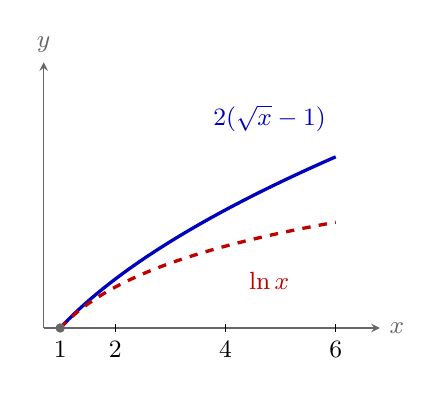
\begin{tikzpicture}[x=0.70cm,y=0.75cm,>=stealth,font=\small]
		\draw[->,gray!80!black] (0.7,0)--(6.8,0) node[right] {$x$};
		\draw[->,gray!80!black] (0.7,0)--(0.7,4.5) node[above] {$y$};
		\foreach \x in {1,2,4,6}{\draw (\x,0.07)--(\x,-0.07) node[below]{\x};}
		\draw[blue!75!black,very thick] plot[domain=1:6,samples=70] (\x,{2*(sqrt(\x)-1)});
		\draw[red!75!black,very thick,dashed] plot[domain=1:6,samples=70] (\x,{ln(\x)});
		\fill[gray!80!black] (1,0) circle (1.7pt);
		\node[anchor=west,blue!75!black] at (3.6,3.55) {$2(\sqrt{x}-1)$};
		\node[anchor=west,red!75!black] at (4.25,.8) {$\ln x$};
	\end{tikzpicture}
